\section{Evaluation Methodology}
\label{sec:evaluation:methodology}

% Talk about standard evaluation methodology and its drawbacks
Even though activity recognition is very diverse in terms of sensor approaches and algorithmic choices, evaluation is usually carried out applying a very well known methodology which can be summarised in the following steps:

\begin{enumerate}
 \item Choose a target environment and deploy sensors to acquire and process information about human activities. 
 \item Select a group of persons who can perform target activities in the prepared environment.
 \item Select a dataset labelling system so datasets generated by users can be used as a ground truth, both for the activity recognition system and the evaluation process.
 \item Run experiments with users and label obtained activity datasets.
 \item Use the same datasets to test the activity recognition system and store the labels produced by it.
 \item Compare the labels of the activity recognition system with the ground truth using appropriate metrics.
\end{enumerate}

% Insert a diagram that shows the standard methodology

Each of the enumerated steps may vary depending on the activity recognition approach and the available resources. The described methodology, which will be called \textit{standard methodology} for the rest of the paper, is the reference for any group working on human activity recognition.

Nevertheless, there are some problems that make very difficult to implement the standard methodology. For instance, (i) it is not always possible to own an environment and install sensors and processing systems, due to economic reasons, (ii) running experiments with human beings imply ethical and legal issues that can slow down the research process or sometimes make it impossible, (iii) dataset labelling systems are not perfect, since most of them rely on users' memory or discipline to annotate every activity carried out, and (iv) regulatory limitations on the use of human subjects prohibit the collection of extensive datasets that can test all scenarios and theories under all circumstances. 

There are several research groups that share the datasets they obtain in their pervasive environments, following different variants of the standard methodology. A Wiki Page called BoxLab\footnote{http://boxlab.wikispaces.com/List+of+Home+Datasets} contains a detailed list of public datasets collected in home environments. It contains a description of deployed sensors, whether it is an annotated dataset and the availability of the dataset. Those public datasets can be a very good alternative for those research groups which cannot run their own experiments. Furthermore, public datasets can also be used for benchmarking different activity recognition systems.

%This paper presents a novel evaluation methodology to overcome the enumerated problems. The methodology has been named \textit{hybrid} because it combines real users' inputs and simulation tools. The key idea is to circulate surveys among target users with the objective of capturing how they perform certain activities of daily living. Using the information collected by surveys, individual scripts are prepared, which are then processed by a synthetic dataset generator tool to simulate arbitrary number of days and generate perfectly labelled datasets of activities. To get as close as possible to real world settings, the synthetic dataset generator uses probabilistic sensor noise models and probabilistic time lapses.

% Present the hybrid methodology and show its need and benefits

\subsection{Analysis of the viability of the standard methodology for the extended activity model learning system}

To evaluate properly the EAM learning system, activity datasets that fulfil several conditions are needed. Namely:

\begin{enumerate}
 \item Contain a lot of samples of different activities to enable a proper learning process. To make data-driven learning a meaningful process, many samples of the same activities are needed, specially to learn noise free activity models. If few samples are available and those samples are affected by noise, it is very difficult for the learning process to distinguish between noisy and noiseless models.
 \item Sensor activations must be labelled in order to provide a solid ground truth. An accurate evaluation process needs an accurately labelled dataset, where all sensor activations produced due to an activity execution are annotated with that activity name, whereas sensor noise is not included in the activity.
 \item Specific objects used for activities have to be monitored (dense sensing scenario). Instead of getting data from context sensors such as thermometers, humidity sensors or even movement sensors, datasets have to contain sensor activations monitoring concrete objects such as cups, dishes, food, etc. in order to be able to produce accurate activity models.
 \item At least some of the activities have to be performed in varied ways to see whether the presented learning process can capture all those variations. Different ways of performing the same activity are needed, since the EAM learning system aims at capturing sub-activities. If all the activities are performed the same way in terms of executed actions, the dataset will only serve to evaluate the learning of complete models, but not specialised models.
 \item Several users are needed as the approach aims at capturing concrete activity models for concrete users. Every user has his/her own way to perform the same activities and one of the objectives of the EAM learning system is to be able to model those personalised models. Thus, to show that the EAM learning system can really deal with different users, datasets of several users are required.
\end{enumerate}

Following the standard methodology to generate such datasets implies a high-cost process with many ethical and legal constraints regarding the use of people for experiments. That cost, both economical and time cost, could not be assumed during the development of the current dissertation. Due to this limitation, public dataset repositories were analysed carefully to find an appropriate dataset.

Unfortunately, datasets that meet all the enumerated conditions could not be found in those public repositories. Some datasets used different activity monitoring approaches, such as vision- and wearable-based monitoring. Some other datasets could be used for the dense sensing scenario since they monitor specific objects, but activities are performed from a list where no variations can be found. Yet other datasets are more focused on monitoring the contextual information, rather than concrete user-object interactions.

As Helal et al. state in their paper \cite{Helal2011}:

\blockquote{\textit{Access to meaningful collections of sensory data is one of the major impediments in human activity recognition research. Researchers often need data to evaluate the viability of their models and algorithms. But useful sensory data from real world deployments of pervasive spaces are very scarce. This is due to the significant cost and elaborate groundwork needed to create actual spaces. Additionally, human subjects are not easy to find and recruit. Even in real deployments, human subjects cannot be used extensively to test all scenarios and verify multitudes of theories. Rather, human subjects are used to validate the most basic aspects of the pervasive space and its applications, leaving many questions unanswered and theories unverified.}}

This is the case of the presented approach for EAM learning. It turns out that there cannot be found datasets from real pervasive environments to verify the exposed theory. However, Helal et al. propose a solution to this problem in the same paper \cite{Helal2011}:

\blockquote{\textit{It is thus necessary to develop alternative and practical approaches to studying human activity recognition. Powerful and realistic simulation tools could be used to support the growing demand for test data. Simulations enable researchers to create focused synthetic replications of important events and activities under study. It can be easily changed and refined allowing researchers efficiently to experiment, analyze and fine-tune their models and associated algorithms. Simulation also allows a wider community of researchers to engage and collaborate to solve a specific problem. Hence, a design based on preliminary simulation studies would most likely to be a more robust and inclusive design. Also, a simulation model that mimics an existing real world pervasive space is most likely to answer more questions (and generate much more data) than the target actual space.}}

Following those ideas simulation tools have already been used for activity recognition. For example,   Okeyo et al. use a synthetic data generator tool to simulate time intervals between sensor activations \cite{Okeyo2012a}. Their research is focused on sensor data stream segmentation, so the tool generates varying patterns of sensor activations in order to verify their approach. Liao et al. combine simulation tools and real data for activity recognition in \cite{Liao2006}. A more elaborated simulator has been developed by Bruneau et al. in \cite{Bruneau2009}: DiaSim. The DiaSim simulator executes pervasive computing applications by creating an emulation layer and developing simulation logic using a programming framework. However, it is more focused on simulating applications such as fire situations, intrusions, etc. to identify potential conflicts. In consequence, DiaSim cannot be directly applied to activity recognition. Finally, Helal et al. propose to develop powerful and realistic simulation tools to study human activity recognition. They develop a simulator called \textit{Persim}, which has been enhanced in the new version \textit{Persim-3D} \cite{Helal2012}. Persim is an event driven simulator of human activities in pervasive spaces. Persim is capable of capturing elements of space, sensors, behaviours (activities), and their inter-relationships. Persim is becoming a very complete simulator tool for activity recognition in pervasive environments. However, it is still under development and one of the main limitations is that it does not provide a way to model realistically human behaviour. Authors have already identified this limitation and they are currently working on programming by demonstration approaches to overcome the problem.

As it can be seen in the literature review done in the paragraph above, simulation tools can be used for activity recognition, since they provide accurate enough datasets to verify some theories. However, none of the references given above specify a concrete methodology to use simulators to evaluate activity recognition approaches. There is no information about how activities should be defined, how different users can be modelled, sensor error models, etc. which are key issues when using a simulator. Therefore, there is a lack of a sound methodology that addresses the usage of simulation tools for activity recognition evaluation. 

\subsection{Hybrid evaluation methodology approach}
\label{subsec:evaluation:hybrid}

\begin{comment}
 - Describe target scenario: dense sensing, single user - single activity
 - Explain in detail the steps: survey, script writing, sensor modelling, synthetic dataset generator 
\end{comment}

The hybrid evaluation methodology has been specially designed for activity recognition systems which assume the dense sensing paradigm (see constraint \ref{cons-dense}). Even though the methodology itself is not limited to concrete scenarios, the implementation presented in this document works for single user - single activity scenarios, i.e. only one user is considered and concurrent or interleaved activities are not taken into account (see constraint \ref{cons-single}). 

The methodology has been named hybrid because it combines real users’ inputs and simulation tools. The key idea is to circulate surveys among target users with the objective of capturing how they perform certain activities of daily living. Additionally, users are also requested to describe how their days are in terms of defined activities. For example, a user might make a coffee and brush teeth in week days between 7:00 and 7:30 AM. So the aim of those surveys is to model real human behaviour, covering one of the major weaknesses of simulation-based evaluation methodologies. Using the information collected by surveys, individual scripts are prepared, which are then processed by a synthetic dataset generator tool to simulate arbitrary number of days and generate perfectly labelled datasets of activities. To get as close as possible to real world settings, the synthetic dataset generator uses probabilistic sensor noise models and probabilistic time lapses.

Based on those constraints and ideas, the proposed hybrid evaluation methodology has the following steps (see Figure \ref{fig-methodology}):

\begin{enumerate}
 \item Design activity surveys: to capture how users perform activities and model their behaviour, a proper survey has to be designed. A detailed explanation of how surveys are designed for this dissertation can be found in Section \ref{subsubsec:evaluation:survey}.
 \item Select target users: depending on the objectives of the research, several user groups can be selected. For example, if the system aims at providing help to elderly people, selecting members of that target group is recommended.
 \item Distribute surveys among target users: a suitable way to distribute surveys has to be used, which guarantees users' anonymity. The distribution method can also be influenced by target users. For example, using web-based surveys can be a bad idea if surveys are directed to elderly people, who can be unfamiliar with those technologies. Personal interviews may be a good alternative for those cases.
 \item Translate surveys to scripts: this step is critical. Appropriate criteria have to be adopted to translate the answers obtained from surveys to scripts for the synthetic dataset generator - or any other simulator -. It is very important not to alter or lose the information provided by users.
 \item Model sensor noise: sensor noise has to be modelled in order to achieve realistic activity datasets. Real sensors are not perfect and depending on their technological base, error models have to be provided.
 \item Run synthetic dataset generator: using the scripts obtained from surveys and sensor error models, the synthetic dataset generator is executed. The output of the tool is a labelled activity dataset which will serve as the ground truth for evaluation.
 \item Develop the activity modelling and/or recognition system: researchers have to develop the activity modelling and/or recognition system in order to be tested. Notice that datasets generated by the synthetic dataset generator can also be used in this step, specially for data-driven approaches.
 \item Compare results: finally, the results obtained by the activity modelling and/or recognition system have to be compared with the ground truth, using appropriate metrics.
\end{enumerate}

\begin{figure}[htbp]
\centering
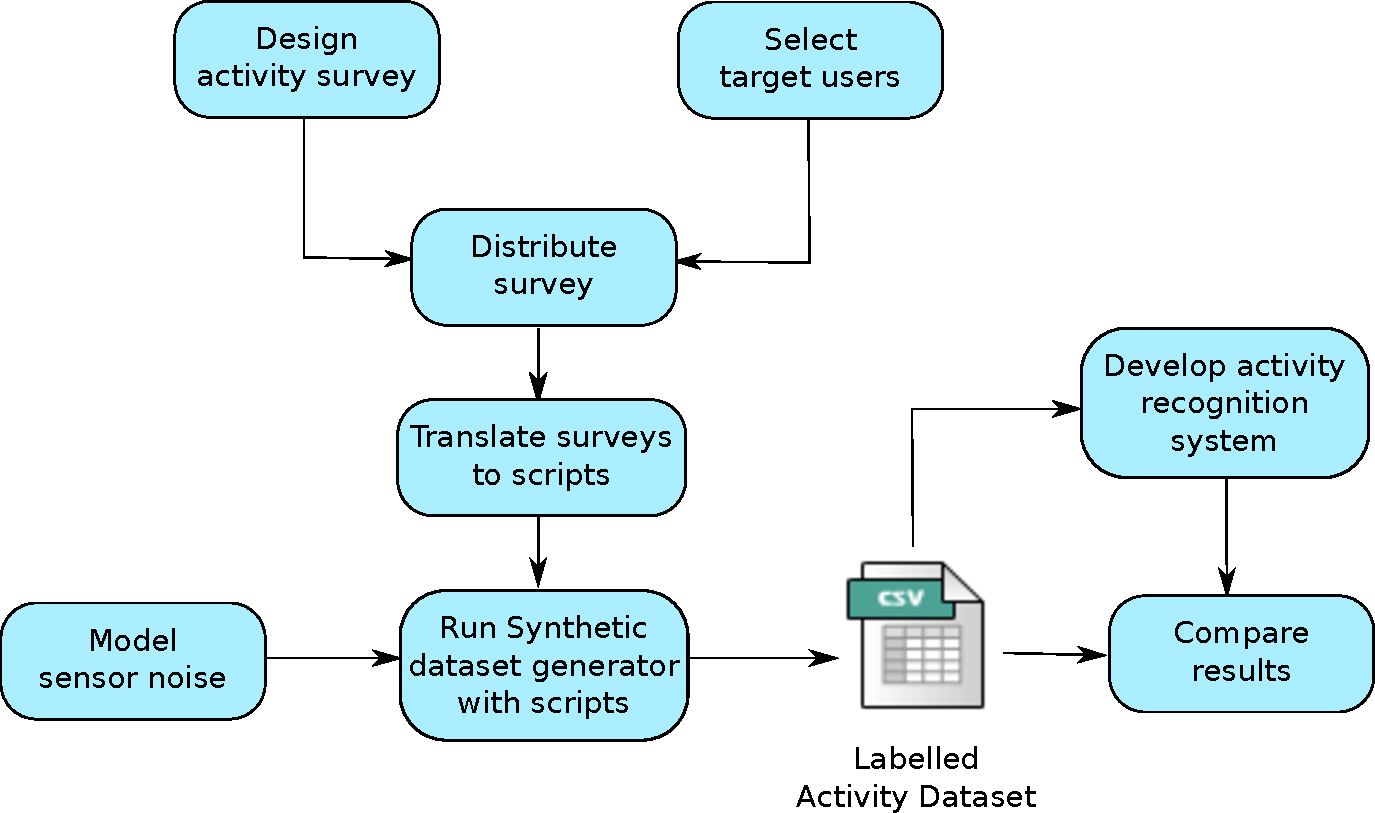
\includegraphics[width=12cm]{hybrid_methodology.pdf}
    \caption{The hybrid evaluation methodology steps depicted in a flowchart.}
    \label{fig-methodology}
\end{figure}

\subsubsection{Survey for activities of daily living}
\label{subsubsec:evaluation:survey}
\begin{comment}
 - Explain each of the questions of the survey
 - Show a screenshot and provide the link to the Google Form
 - Google Forms guarantee users' anonymity
 - Explain survey-script translation criteria
\end{comment}

One of the main advantages of considering dense sensing scenarios is that activities are described in terms of the objects which have been used to perform that activity. Furthermore, as only sensor activations (and not de-activations) are important for the approach (see definition \ref{def-sa}), to model an activity, it is enough to know which objects are used by the user and the order of usage of those objects. This information is easy to obtain in a survey and will be named \textbf{activity model}.

\begin{defn}[Activity model]
\label{def-act-model}
 An activity model is a sequence of objects used by a user to perform an activity. A user might provide more than one activity models per defined activity, because the same activity can be performed in several ways. Activity models also provide a typical duration given by the user.
\end{defn}

On the other hand, to model human behaviour appropriately, acquiring activity models is not enough. It is very important to know what activities are performed by a concrete user in a daily basis, alongside with the time slots and time lapses between contiguous activities. 

\begin{defn}[Behaviour model]
\label{def-behaviour}
 A behaviour model is a sequence of activities with associated time slots and time lapses. A user might provide several behaviour models, as every day can be different in terms of performed activities and times.
\end{defn}

The main objective of the survey is to obtain activity and behaviour models from target users. Hence, the survey for activities of daily living has two main parts. The first part is devoted to capture what activities are performed in different days, i.e. behaviour models. The second part, on the other hand, asks users about how they perform those activities based on user-object interactions, i.e. activity models. The concrete survey used for the experiments carried out in this dissertation can be found in the web\footnote{http://goo.gl/etCNyi}. 

As it can be seen in Figure \ref{fig-survey-1}, the survey begins with a brief explanation for target users, where the aims of the survey are stated and the target activities are presented. In this case, target activities are seven: make a coffee, make a chocolate, make pasta, brush teeth, watch television, wash hands and read a book. Afterwards, under the heading of ``Day Description'', users are asked to describe their week days in terms of activities. They are expected to provide information about time slots and activity sequences performed in those time slots. Users are also asked to provide time relations between two consecutive activities. For example, between 7:00 and 7:30 AM a user might make a coffee and ten minutes later might brush teeth. This first part has been designed to obtain behaviour models for target users.

\begin{figure}[htbp]
\centering
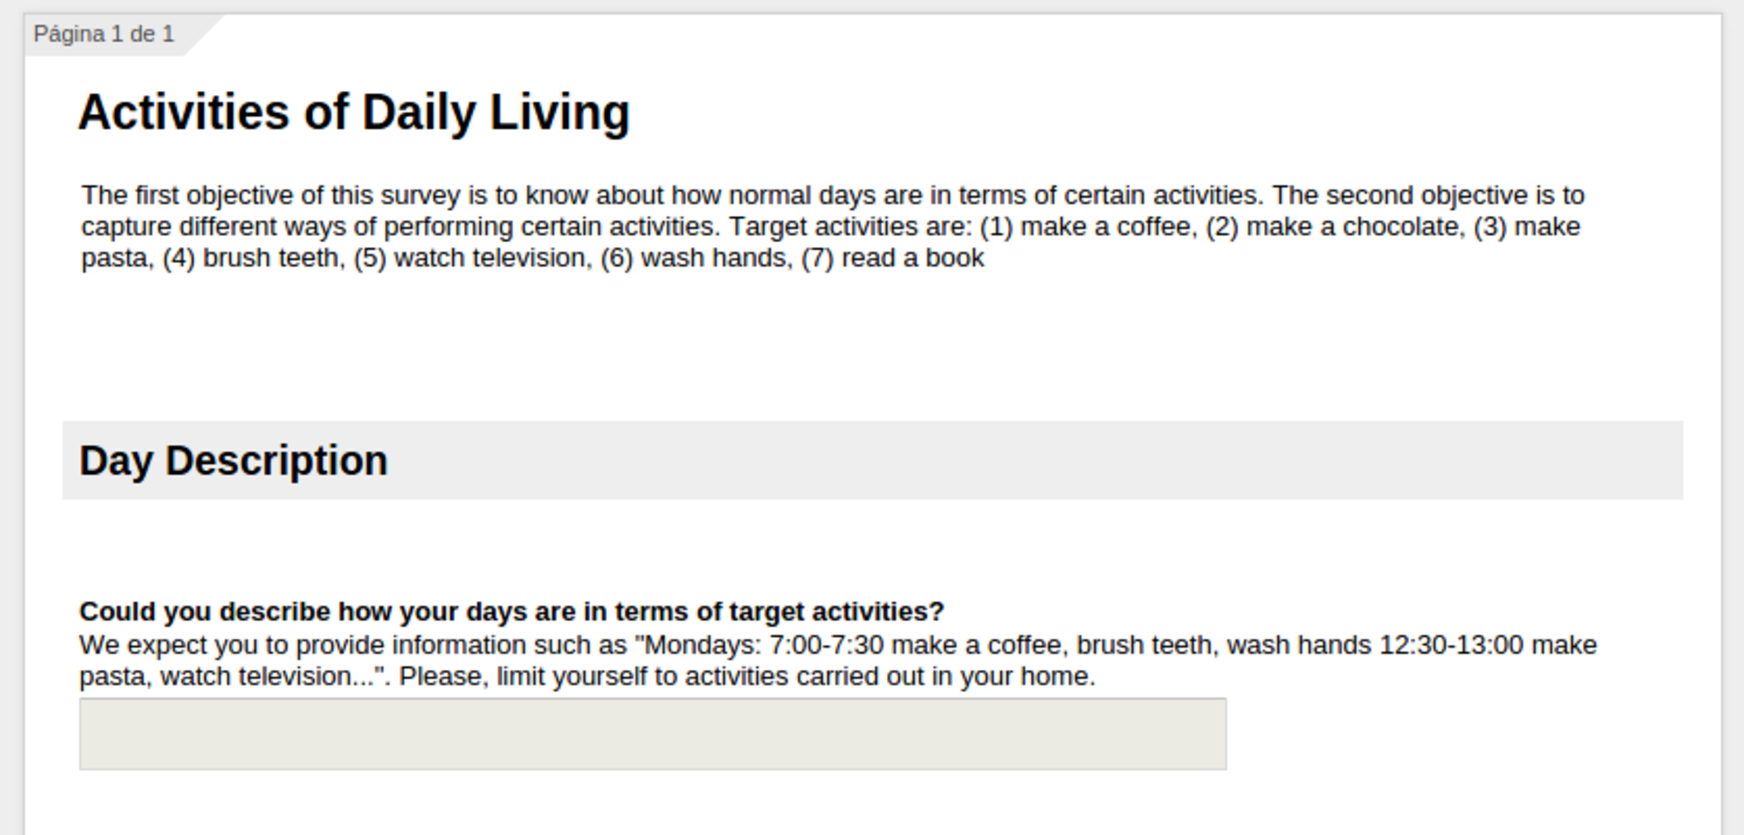
\includegraphics[width=\textwidth]{adl_survey_part1.pdf}
    \caption{The first part of the survey. A small introduction can be found where the aim of the survey is explained, continuing with the behaviour model part.}
    \label{fig-survey-1}
\end{figure}

The second part of the survey is longer. Target activities are presented one by one. For each activity, several questions are asked to users, to capture the locations of activities, the ways activities are performed, the objects used for each activity, a description of how those objects are used and typical duration estimations. An example of those questions can be found in Figure \ref{fig-survey-2} for the activity MakeCoffee.

\begin{figure}[htbp]
\centering
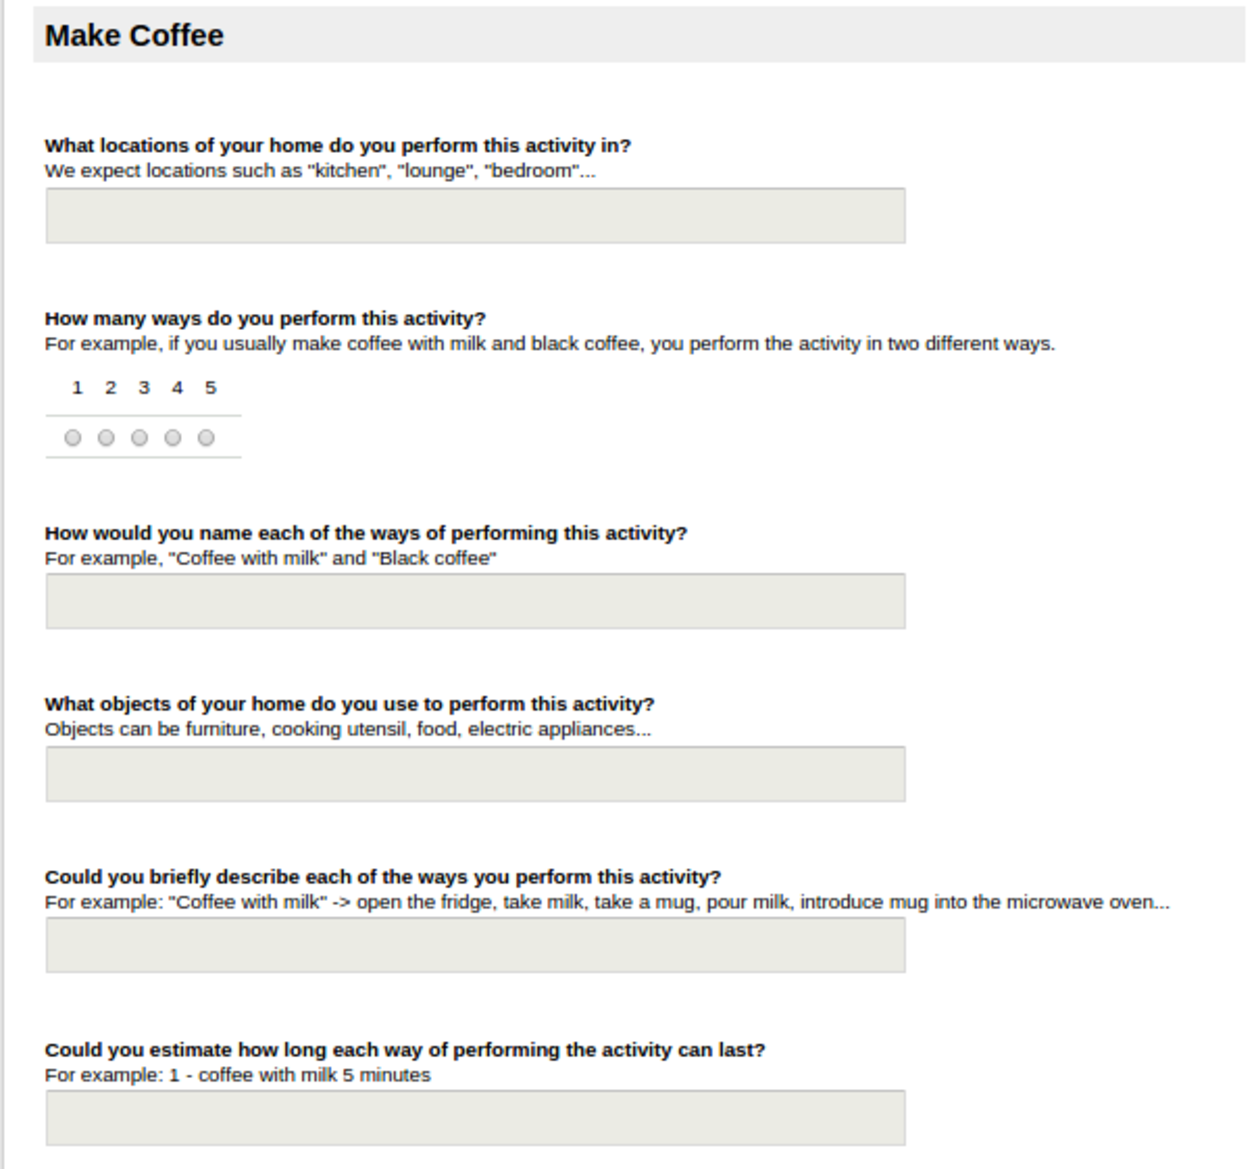
\includegraphics[width=\textwidth]{adl_survey_part2.pdf}
    \caption{The questions of the survey to capture the activity model of MakeCoffee.}
    \label{fig-survey-2}
\end{figure}

As Figure \ref{fig-survey-2} shows six questions are asked per activity. The first question is to know where the activity is performed by the user. As stated in the brief explanation under the question, expected locations are home locations such as kitchen, lounge, etc. Each activity may be performed in several locations, in concordance with the context knowledge model shown in Figure \ref{fig-context-json}. Notice also that expected locations fulfil with the location definition given in definition \ref{def-location}.

The second question deals with different ways of performing an activity, i.e. sub-activities. Users are asked to provide a variation name, which will define the name of the sub-activity. The next question asks about the objects used to perform the activity. This will serve not only to model the activity itself, but also to model the context knowledge, where objects and attached sensors are represented (see Section \ref{subsec:approach:inputs}). Afterwards, the most important question for activity modelling comes: a description of how the enumerated objects are used to perform the activity. Descriptions are requested for each activity variation. From those descriptions, object usage order and time lapses will be obtained. Finally, the last question aims at modelling typical durations for the variations of the target activity.

As described in the steps of the hybrid evaluation methodology in Section \ref{subsec:evaluation:hybrid}, it is also important to decide the way to circulate the survey and to guarantee user anonymity. In our current experiments, we use Google Forms\footnote{http://www.google.com/google-d-s/createforms.html}, mainly for three reasons:

\begin{enumerate}
 \item Easy circulation: surveys can be sent by e-mail to target users, who receive a link to the web-based survey. This makes survey circulation easy and clear.
 \item Anonymity: the answers of users are completely anonymous. When a user submits his/her answers, only a tag like ``user 1'' appears. There is no way to link user answers to a concrete user.
 \item Simple and centralised answer management: Google Forms service generates a centralised table where all the answers are collected. The table is automatically updated whenever a new answer arrives. This web-based table system for answers make data management much easier.
\end{enumerate}

Summarising, the survey for activities has different questions in order to obtain activity and behaviour models according to their definitions (definitions \ref{def-act-model} and \ref{def-behaviour}). Surveys are circulated among target users using Google Forms, which offers convenient tools to send them by e-mail and collect anonymous answers in a centralised manner.


% We may introduce some snapshots of the survey to explain what we wan to obtain from that part

%%%%%%%%%%%%%%%%%%%%%%%%%%%%%%%%%%%%%%%%%%%%%%%%%%%%%%%%%%%%%%%%%%%%%%%%%%%%%%%%%
%%%%%%% SYNTHETIC DATASET GENERATOR
%%%%%%%%%%%%%%%%%%%%%%%%%%%%%%%%%%%%%%%%%%%%%%%%%%%%%%%%%%%%%%%%%%%%%%%%%%%%%%%%%
\subsubsection{Synthetic dataset generator}
\label{subsubsec:evaluation:synthetic}
\begin{comment}
 - Explain the script: sensor activation patterns, activity patterns (sequences and alterations), sensor positive noise
 - Explain probabilistic sensor modelling
 - Explain probabilistic time lapses
 - Show output examples and give numbers
\end{comment}
Although the hybrid methodology for evaluation could be used in principle with any simulator for human activity recognition, a custom simulation tool has been developed to evaluate the EAM learning system. Available simulators such as Persim do not cover all the conditions to evaluate the EAM learning system appropriately. It may be very useful in the future, but nowadays it does not have the tools to model sensor errors and different variations of activities.

Following the ideas of Okeyo et al. \cite{Okeyo2012a}, instead of developing a simulator tool that provides visual interaction like Persim, a synthetic dataset generator has been developed. The tool presented by Okeyo et al. does a very good job simulating time relations between sensor activations and activities, so their ideas regarding time management have been borrowed. But the simulator tool developed for this dissertation has more capabilities, allowing researchers to introduce different sensor activation sequences for activities with occurrence probabilities, activity sequences which occur only with a given probability and different ways to model sensor errors.

The synthetic dataset generator tool has been implemented in Python 2.7\footnote{https://www.python.org/}. The inputs to the synthetic dataset generator are a script called ADL script, where activity and behaviour models for a concrete user are represented, and the context knowledge file, where some sensor error models are provided. As sensor error models are linked to their type (pressure, tilt, contact, etc), it is a natural choice to place them where all the sensors of a concrete environment are represented, i.e. in the context knowledge file. This part of the context knowledge file has not been introduced in Section \ref{subsec:approach:inputs} because it was not important for the EAM learning system. However, for simulation purposes, sensor error models play a crucial role, and including them in the context knowledge file was the straightforward solution. Considered sensor error modalities are two: sensor positive noise (see definition \ref{def-positive}) and missing noise (see definition \ref{def-missing}).

Figure \ref{fig-synth-tool} shows a high-level design for the synthetic dataset generator. As it can be seen in the figure, activity and behaviour models and sensor positive noise are represented in the ADL script. On the other hand, sensor missing noise models are obtained from the context knowledge file. Using probabilistic time management tools, the synthetic dataset generator creates a sensor activation dataset, where all sensor activations are properly labelled to use it as ground truth. Sensor activations which are part of an activity are labelled with the activity name. But sensor activations which appear due to sensor noise are labelled with the special label None. 

\begin{figure}[htbp]
\centering
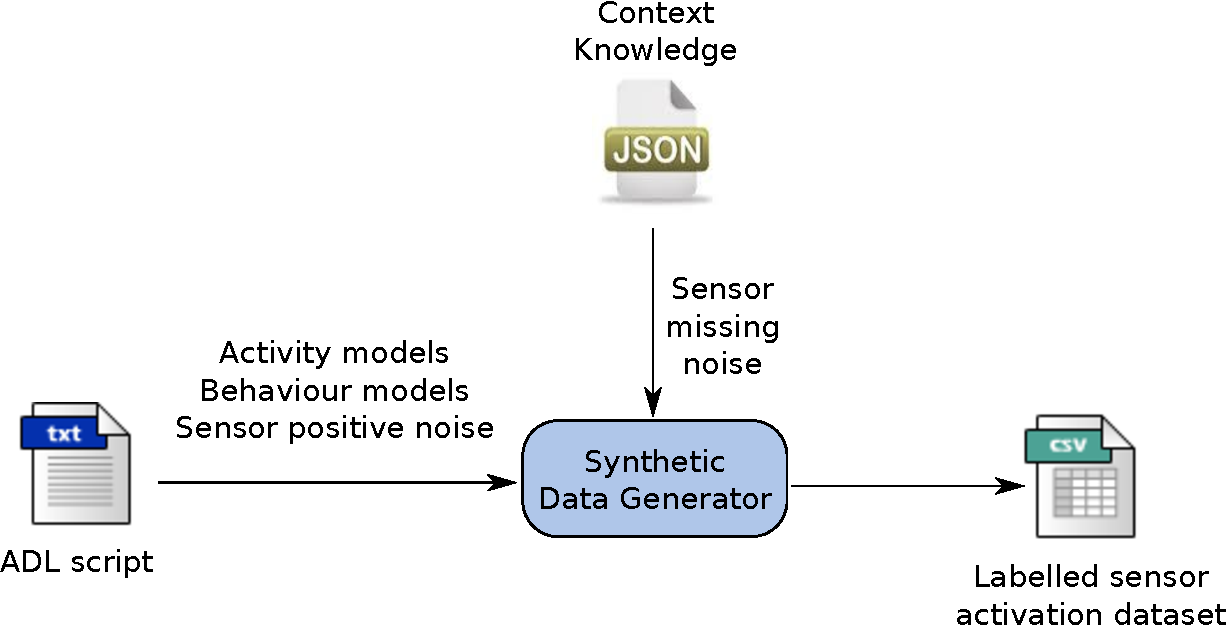
\includegraphics[width=10cm]{synthetic_tool.pdf}
    \caption{High-level design of the synthetic dataset generator tool.}
    \label{fig-synth-tool}
\end{figure}

One of the design decisions was to separate the representation of both sensor error models between two different files. The reason is that sensor missing noise is completely linked to sensor technology and the pervasive infrastructure (wireless receivers, communication, and system sampling and conversion mechanisms), whereas sensor positive noise is more related to environmental aspects, such as the distribution of objects and human behaviour. Hence while sensor missing noise can be considered a property of a sensor, sensor positive noise is more influenced by the inhabitant and the environment. That is why missing error models are included in the context knowledge file depending on the sensor type and positive error models are represented in the ADL script which represents a concrete user.

To make this decision the research carried out by Chen et al. in \cite{Chen2012a} has been considered. They show some experiments for activity recognition in a smart home environment using the dense sense activity monitoring approach. Throughout the experiment of 144 activities, a total of 804 user-object interactions were performed. They used the so called User-object Interaction Recognition Accuracy (UoIR), defined as the system’s correctly captured interactions against the total occurred interactions, as the metric to evaluate the reliability and performance of the activity monitoring mechanism. This metric takes into account not only unfired or misread interactions caused by faulty sensors but also those circumstances caused by pervasive infrastructure. As such it is more accurate to reflect the system monitoring performance. Table \ref{tab-sensor-errors} shows the UoIR for different types of sensors with an overall average UoIR of 96.89\%. They conclude that this data proves the monitoring and acquisition mechanism of the system as being very reliable.

\begin{table}[htbp]\scriptsize
\begin{center}
 \begin{tabular}{cccc}
  \hline
  Sensor type & Total interactions & Captured interactions & Accuracy (\%) \\
  \hline
  Contact & 624 & 611 & 97.92 \\
  Tilt & 126 & 119 & 94.44 \\
  Pressure & 36 & 32 & 88.89 \\
  Sound & 18 & 17 & 94.44 \\
  \hline
 \end{tabular}
 \caption{Interaction recognition rate as shown in \cite{Chen2012a}.}
 \label{tab-sensor-errors}
\end{center} 
\end{table}

However, no positive sensor noise has been identified in \cite{Chen2012a}, even though they simulate it in some of their experiments. This is quite reasonable, since the normal state of the sensor represents no interaction. It is very complicated from the technological point of view to change the state of a sensor when no interaction occurs, so it can be concluded that spontaneous sensor activations are very rare. If positive sensor noise is registered, it has to be mainly caused by undesired interactions that actually occur, even though they are not part of the activity. Those undesired interactions can be due to human erratic behaviour (see definition \ref{def-erratic}) or interactions among objects caused by their distribution and casual movements. 

As according to literature spontaneous sensor activations are rare and interactions among objects usually occur due to human intervention, it can be concluded that sensor positive noise is mainly caused by user erratic behaviour. Thus it has been included in the ADL script rather than in the contextual knowledge file.

\subsubsection*{ADL script}

The ADL script defines activity models, behaviour models and sensor positive noise for a concrete user. It is currently implemented as a plain text file which has its own syntax. A parser function has been implemented to parse the file and obtain all the models defined on it. 

The first information given in the ADL script refers to the number of days that has to be simulated. A natural number is provided there.

The next part of the file is for defining \textit{sensor activation patterns} for activities. Sensor activation patterns are used to describe how activities are performed in terms of sensor activations and thus represent activity models in terms of sensors. An activity can have an arbitrary number of sensor activation patterns, which are specified with an occurrence probability and a sequence of sensor activations with relative time lapses. An example of sensor activation patterns for activity MakeCoffee can be found in Figure \ref{fig:sensor-act}.

\begin{figure}
\begin{small}
\lstset{linewidth=\textwidth}
\begin{lstlisting}
MakeCoffee 2
0.7 coffeePotSens@0 ktapSens@10 afcoffeeSens@30 cookerSens@20 
    cupSens@180 fridgeSens@10 smilkSens@5 wsugarSens@10
0.3 coffeePotSens@0 ktapSens@10 afcoffeeSens@30 cookerSens@20 
    cupSens@180 wsugarSens@10
\end{lstlisting}
\end{small}
\caption{Sensor activation patterns for MakeCoffee activity obtained from a real user. The activity has two activation patterns with different occurrence probabilities.}
\label{fig:sensor-act}
\end{figure}

First of all, the name of the activity is defined. The number that comes after the name specifies the number of sensor activation patterns for that activity. The next line represents the first sensor activation pattern, which begins with an occurrence probability $p \in [0, 1]$. Notice that the occurrence probabilities of all sensor activations for a given activity must sum to 1. The probability number is followed by a sequence of sensor activations and relative time lapses. The first sensor activation's time has to be 0, indicating that it is the first sensor activation of the activity. The values that come after the '@' symbol represent the time in seconds between the previous sensor activation and the current one. In consequence, in the example given in Figure \ref{fig:sensor-act}, \textit{cookerSens@20} means that sensor activation \textit{cookerSens} occurs 20 seconds after the \textit{afcoffeeSens} sensor activation. How the synthetic dataset generator treats those time lapses will be explained later, when the simulation loop is described.
%The synthetic dataset generator establishes a time lapse with a Gaussian random generator whose mean value is the value specified in the script and the standard deviation is the 25\% of the mean. This way, time lapses between two consecutive sensor activations are realistic. 

Once all activity models are represented using appropriate sensor activation patterns, behaviour models are defined, which represent different days of the user in terms of performed activities (see definition \ref{def-behaviour}). Two kinds of behaviour models are defined: 

\begin{enumerate}
 \item \textbf{Sequences:} where a time slot is given with a sequence of activities and relative time lapses between two consecutive activities. Sequences are used to define those activity sequences that are always performed by a user in concrete days.
 \item \textbf{Alterations:} where a probability value is assigned to an activity to be performed in a concrete time slot. Alterations represent a different kind of behaviour model. Some users might perform an activity regardless of the week day. For example, a user might watch television in evenings with a certain probability. Some days the user watches television, but some days does not. It does not depend on the day, but on some other causes (mood, last hour plans, etc.).
\end{enumerate}

Specific week days are not represented in behaviour models. Instead of that, the probability of a concrete list of sequences and alterations is given. A list of sequences and alterations model a day. So if such a day model occurs 2 days in a week, i.e. in weekends, the assigned probability will be $2/7 \simeq 0.29$. An example is depicted in Figure \ref{fig:activity-pattern}. A typical day of a user is described, with an occurrence probability of 0.29, since the activity pattern describes a weekend day. In this case, the user reported that (s)he sometimes reads a book in the afternoon. Alterations allow modelling this kind of behaviour.


\begin{figure}
\begin{small}
\lstset{linewidth=\textwidth}
\begin{lstlisting}
Prob 0.29 4
S 9:00-10:00 MakeCoffee@0 BrushTeeth@1800 ReadBook@120
S 13:30-14:30 MakePasta@0 BrushTeeth@600
S 22:00-23:00 BrushTeeth@0 WashHands@10
A 18:00-20:00 ReadBook 0.5
\end{lstlisting}
\end{small}
\caption{An example of a behaviour model for a concrete day, which has an occurrence probability of 0.29 and it is composed of three sequences and an alteration.}
\label{fig:activity-pattern}
\end{figure}

As it happens with sensor activation patterns, the occurrence probabilities of behaviour models must sum to 1.

The last part of the script is to define sensor positive noise (see definition \ref{def-positive}). As sensor positive noise is mainly caused by user erratic behaviour it is very complex to model it accurately. Besides, obtaining those models from user surveys is impossible, since users cannot tell how they interact with objects unpurposely. For those reasons, a simple sensor error model has been adopted which guarantees noise generation independently from ongoing activities. A probability value can be assigned to concrete sensors to get activated in an hour interval using a uniform probability distribution. For example, sensor \textit{cupSens} can be assigned an activation probability of 0.1, which means that each hour, the sensor has a 0.1 probability of getting activated. 

\subsubsection*{Context knowledge file}

The context knowledge file has been described in Section \ref{subsec:approach:inputs}, where an example of such a file was provided in Figure \ref{fig-context-json}. But sensor missing noise models were not shown in that example. As sensor missing noise is mainly related to the sensor type, another part is added to the context knowledge file. More concretely, Figure \ref{fig-missing-noise} shows an example of how such error models are implemented for contact and tilt sensors. For each sensor type, a missing probability $p \in [0, 1]$ is provided. 

\begin{figure}[htbp]
\begin{small}
\begin{lstlisting}
"error_models": {
   "contact": {
	"prob": 0.0208
   },
   "tilt": {
	"prob": 0.0556
  },
  ...
}
\end{lstlisting}
\end{small}
\caption{Example of sensor missing noise models for contact and tilt sensors.}
\label{fig-missing-noise}
\end{figure}

In consequence, the context knowledge file has the information about activities, objects, sensors and sensor missing noise models. It is mandatory for the synthetic dataset generator to keep the coherence between the sensors used in the ADL script and in the context knowledge file. The tool itself makes sure that coherence exists. If there is a sensor activation in the ADL script which is not represented in the context knowledge file, the synthetic dataset generator raises an error.

\subsubsection*{Simulation loop}

Using the ADL script and the context model file, the synthetic dataset generator creates a CSV file where each sensor activation has an associated time-stamp and is labelled with an activity name or with the special label None if it is caused by noise. Additionally, activity start and end time are marked in the dataset.

For that purpose, the synthetic dataset generator has a simulation loop which has been represented in a flowchart in Figure \ref{fig-sim-loop}. First of all, the simulator fixes the first day to start the simulation. In the current implementation the same day the simulator is launched is used as the first day. Afterwards, for the selected day, sensor positive noise is generated. For that purpose, the simulator generates a random number per each sensor with a probability greater than zero. If the sensor has to be activated, the simulator chooses a concrete time inside the current hour using a uniform distribution. The process finishes when the 24 hours of the day have been treated.

\begin{figure}[htbp]
\centering
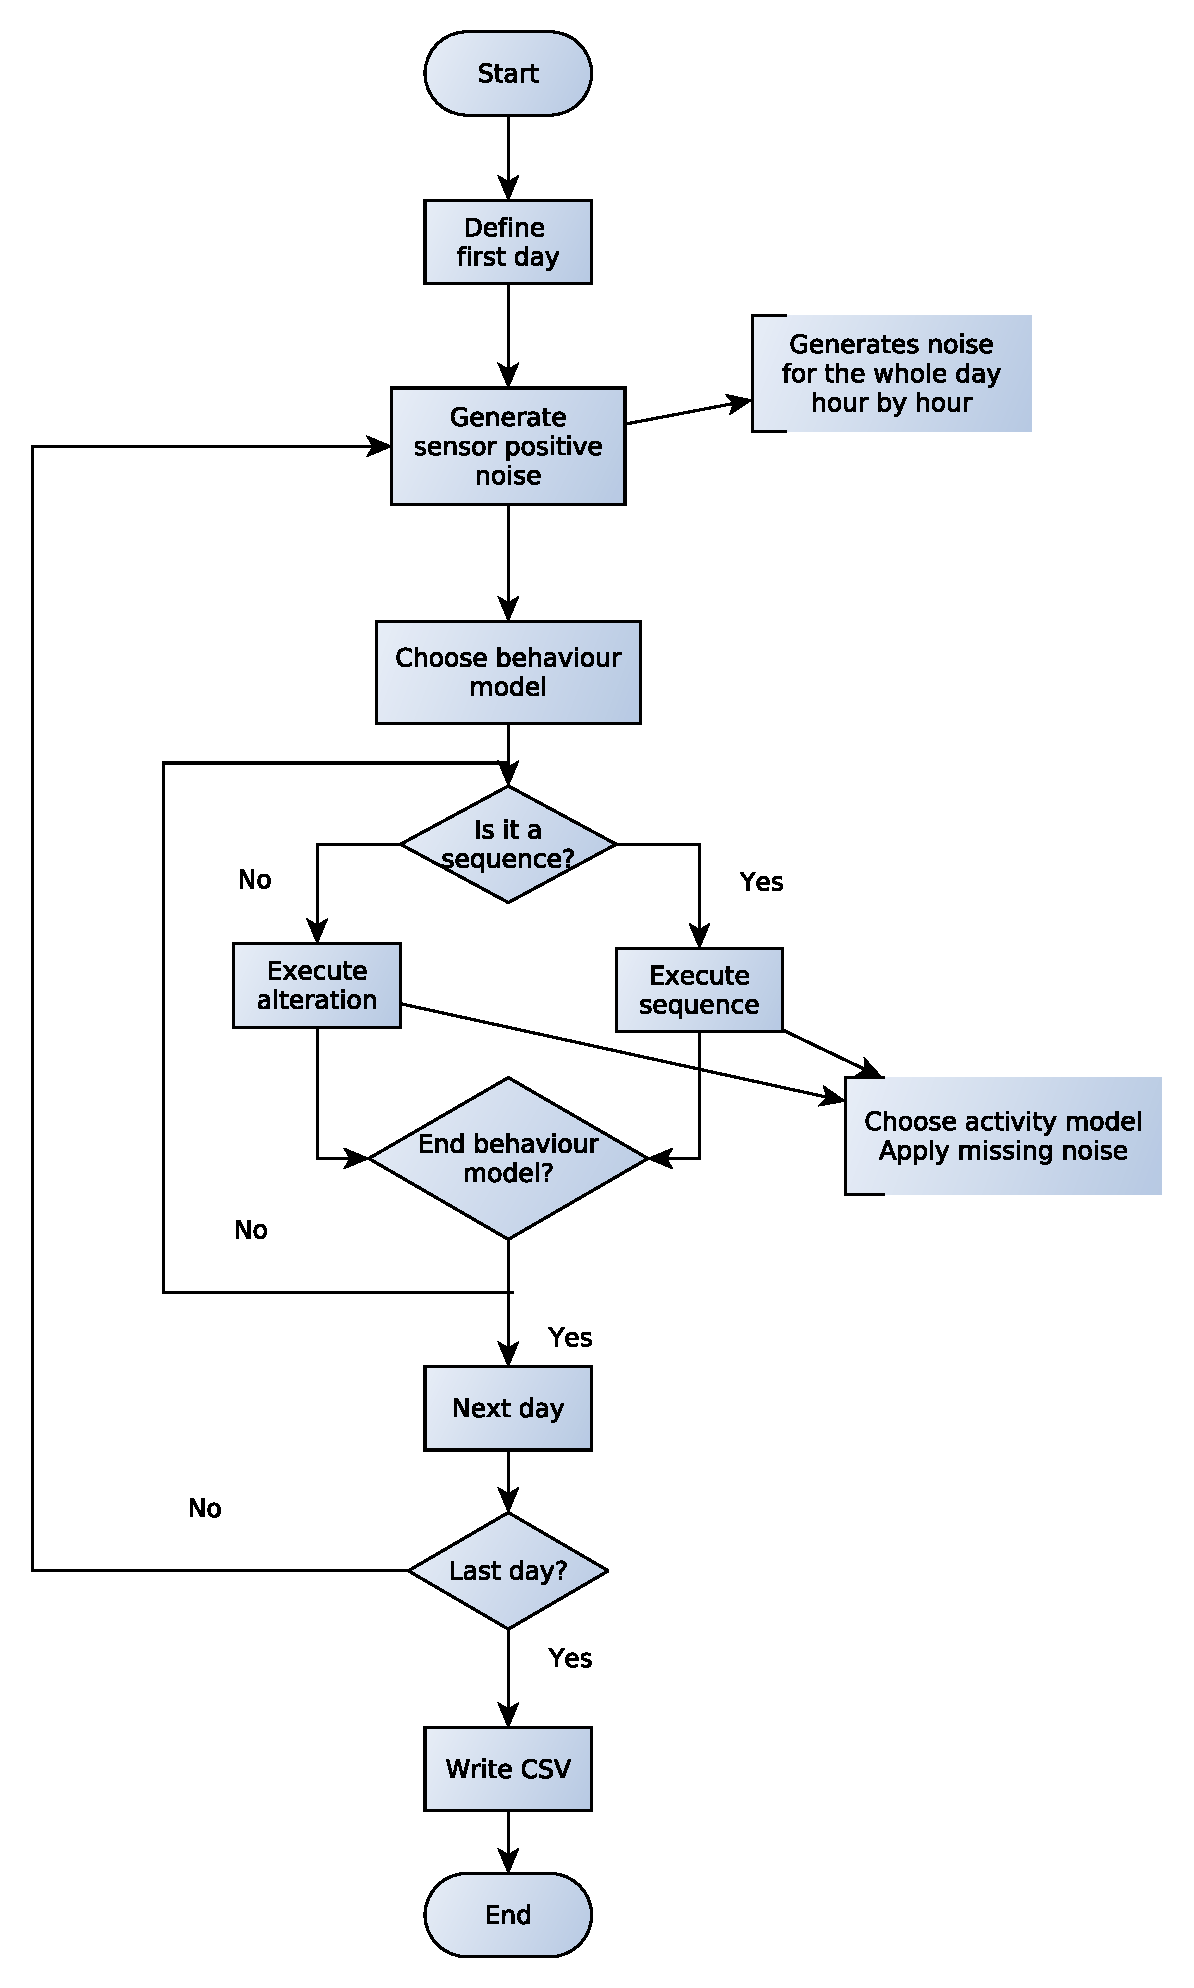
\includegraphics[width=11cm]{simulation_loop.pdf}
    \caption{A flowchart of the simulation loop of the synthetic dataset generator.}
    \label{fig-sim-loop}
\end{figure}

Once sensor positive noise has been generated for the whole day, a behaviour model is chosen, taking into account the probabilities of each model. The behaviour model is a list of sequences and alterations. The first element of the list is taken. If it is a sequence, the activities of the sequence are executed in the specified time slot. For example, assume the sequence is such that 

\begin{small}
\begin{lstlisting}
 S 9:00-10:00 MakeCoffe@0 WatchTelevision@30 BrushTeeth@1800 
\end{lstlisting}
\end{small}

\noindent In that case, the simulator generates a start time for the sequence in the provided time slot, using a uniform distribution. Afterwards, it picks the first activity (MakeCoffee) and looks for the sensor activation patterns of that activity. The simulator probabilistically chooses one of the sensor activation patterns of the activity and executes it. While executing the activity itself, two main aspects are taken into account:

\begin{enumerate}
 \item Time lapses between sensor activations: the numbers provided in the script are used as the mean value of a Gaussian distribution, whose standard deviation is fixed to a 25\% of the mean by default. So the time lapse is generated probabilistically using as reference the value given in the script. This makes varying and realistic time lapses for consecutive sensor activations.
 \item Sensor missing noise: before generating the sensor activation, its missing probability is consulted in the context file. The simulator uses the missing probability to decide whether to generate the activation.
\end{enumerate}

Similarly to sensor activations, time lapses between activities are treated through Gaussian distributions. At the end of the process, the whole sequence will be executed, with probabilistically chosen time lapses and sensor missing errors.

To execute an alteration, the simulator uses its occurrence probability. If it has to be executed, the activity is performed as in sequences. When the behaviour model is fully executed, i.e. all the elements of the list have been treated, the simulator generates the next day and repeats the whole process until the last day is reached. When this happens, the generated dataset is written in a CSV file, where properly labelled time-stamped sensor activations can be found.

\subsection{Discussion about the hybrid methodology}
\label{subsec:evaluation:hybrid:discussion}
\begin{comment}
- Explain the advantages: generate virtually infinite datasets, arbitrary number of days, perfectly labelled, sensor noise, erratic behaviour, realistic time lapses
 - Explain the main disadvantages: erratic behaviour difficult to capture
 \end{comment}
The hybrid methodology explained in Section \ref{subsec:evaluation:hybrid} is based on the literature and has been specially designed to evaluate the EAM learning system and thus, it has some specific tools to adapt the methodology to the constraints of the system. However, the methodology itself, apart from concrete implementations, can be used to evaluate other activity recognition systems and has several advantages over the standard methodology explained in the beginning of Section \ref{sec:evaluation:methodology}. Let us enumerate and justify the advantages:

\begin{enumerate}
 \item The hybrid methodology is cost effective, both from economic and time perspectives: from the economic point of view, the hybrid methodology does not need any pervasive environment, which can become an important investment. Furthermore, the cost of the experiments is also avoided, such as paying to participants, preparations etc. From the time point of view, savings can be very important too, specially if a high number of experiments is planned. Preparing, distributing and processing surveys among users needs a variable amount of time, but it is unarguably less than preparing and running real experiments with humans. 
 \item A lot of users' information can be used: as it is based on surveys, it is generally easy to achieve a great number of users for the tests, in contrast with what happens using the standard methodology. When running experiments with humans, finding volunteers is usually very difficult, specially if the experiment is long in time. 
 \item Ethical and legal issues are much softer: as there are no experiments with human beings many ethical and legal aspects can be avoided. The only important point to be considered is the anonymity of users regarding the information they provide in the surveys.
 \item Datasets can be generated on demand: using the synthetic dataset generator, arbitrary number of datasets can be generated as needed.
 \item Perfectly labelled datasets can be obtained: the synthetic dataset generator labels all sensor activations according to the given script and sensor error models. In consequence, the generated dataset is a perfect ground truth. On the other hand, when using the standard methodology, dataset annotation is a real issue. As noted by Rashidi and Cook in \cite{Rashidi2011}: \blockquote{\textit{An aspect of activity recognition that has been greatly under-explored is the method used to annotate sample data that the scientist can use to train the activity model.}} Several annotation methods have been used by researchers, but all of them have their weaknesses. As a consequence, those datasets are not perfectly labelled and they can include spurious sensor activations in activities as ground truth.
 %\item The influence of researchers is minimised: using surveys, researchers cannot write their own scripts with their bias. Even though researchers are still responsible of writing the scripts, following appropriate survey-script translation criteria, researchers' influence in the datasets is minimised.
 \item Any kind of scenarios can be implemented: the synthetic dataset generator allows preparing experiments where no sensor noise exist, where only a concrete kind of sensor noise exists or where conditions are as close as possible to realistic settings. The chance of implementing all those varieties of scenarios allows researchers test deeper their activity recognition systems, since they can see the influence of any factor they consider relevant. 
\end{enumerate}

The core ideas of the hybrid methodology are using surveys to capture user behaviour and simulators to generate synthetic data. The concrete implementations for the EAM learning system are derived from the constraints and features of the system, such as focusing on dense sensing scenarios, single user - single activity scenarios, etc. However, when constraints are different, different tools can be used inside the same evaluation methodology. 

In this case, the constraints and features of the EAM learning system make feasible the usage of surveys and simulators. The dense sensing paradigm for activity monitoring establishes that user-object interactions are monitored through simple sensor activations, which are used for activity modelling. So sensor activations are boolean valued, making simulation much easier. For example, Persim introduces sensor value generation functions, because the simulated sensors are broader and can produce different values depending on the context. 

Another simplification comes from the activity modelling approach, which is based on action sequences mapped from sensor activations which monitor objects. This means that sensors like thermometers, humidity sensors, etc. do not have to be modelled and simulated for the EAM learning system. Only sensors attached to objects. The same activity modelling approach makes feasible obtaining accurate activity models from users, since it is easy for any user to describe what objects are used to perform activities. 

The single user - single activity constraint also simplifies the whole evaluation process. Firstly, users do not have to provide information about overlapping and concurrent activities, which is very complicated. Additionally, activity models and behaviour models are kept simple for simulation. Modelling and simulating concurrent activities is a challenge that is avoided in this case. 

Finally, time lapses between actions and activities can also be simulated appropriately, as shown by Okeyo et al. \cite{Okeyo2012a}. Users report approximate time lapses in the surveys and the synthetic dataset generator uses Gaussian random number generators in order to generate user based varying time lapses. 

However, there are some disadvantages too and they are mainly related to human behaviour modelling. The first handicap is that modelling user erratic behaviour is complex. It is very difficult for any user to specify what objects (s)he interacts with unpurposely or to say how an activity is aborted because another thing has to be done. The synthetic dataset generator offers a very straightforward way to model this kind of interactions, but it is the researcher who has to assign probability values to specific sensors without having an appropriate way to model user erratic behaviour. The strategy followed in this dissertation is to introduce high levels of random positive noise to compensate the lack of appropriate models. As it will be shown in Section \ref{sec:evaluation:scenarios}, the difference in the number of sensor activations between noiseless and noisy scenarios are around 45\% in average, which means that introduced sensor positive noise is almost a half of the original dataset. 

Another disadvantage refers to the information provided in surveys regarding activity models. Some users are very precise in their answers, but some are not. Activity descriptions given by some users might be discarded due to their vagueness. But this is not generally a big problem, since obtaining more answers is usually easy. Some other users may omit important details of activities in their answers, forgetting for example an object which has been used, hence the precise way of performing activities cannot always be captured. This is certainly a problem while modelling activities, but from the EAM learning evaluation perspective, it is a minor problem. The aim of the EAM learning system is to learn activity models which are represented in the datasets. Whether those datasets are really an accurate version of an activity is not that important as far as the learning system captures and models them as they appear.

In consequence, it can be claimed that the hybrid evaluation methodology with its current implementation, is appropriate to evaluate the proposed EAM learning system. Its advantages are many and very important, while the disadvantages can be coped with specific strategies. 

